% This is not necessarily in the format for a VUW thesis chapter.

% Finished 

\documentclass[a4paper]{report}

\usepackage{amssymb, amsmath}
%\usepackage{mathtools}
\usepackage{tikz}
\usetikzlibrary{calc}
\usepackage{url}

%\usepackage{marvosym}

\newcommand{\beff}{\ensuremath{b_{\mathrm{eff}}}}
\newcommand{\bmin}{\ensuremath{b_{\mathrm{min}}}}
\newcommand{\bmax}{\ensuremath{b_{\mathrm{max}}}}

\newcommand{\blo}{\ensuremath{b_{\mathrm{low}}}}
\newcommand{\bhi}{\ensuremath{b_{\mathrm{high}}}}


\title{Chapter 8: Conclusion}
\author{Nat Lund}


\begin{document}
\maketitle

\subsection*{Summary}

In this PhD thesis we studied the effective slip length of Stokes flow over rough heterogeneous surfaces.  In our mathematical model, the rough surface is modelled as a periodic function $h(x,y)$, and the local intrinsic slip length is modelled as a periodic function $b(x,y)$.  The period $L$ of both functions is the same.  The slip function $b(x,y)$ has a minimum $\bmin$ and a maximum $\bmax$.

Using the homogenization technique for partial differential equations, we showed that if $L < \bmin$, then the effective slip length is the harmonic mean of intrinsic slip lengths, weighted by area of contact between fluid and surface:

\begin{equation}
\beff = \left< \frac{\sqrt{1+ |h'|^2}}{b(x,y)} \right>^{-1}
\end{equation}

We tested this formula against a numerical simulation using finite element methods.  The FEM results show excellent agreement with our prediction if $L \ll \bmin$, and are even within 5\% of our prediction when $L \sim \bmin$.

\vspace*{1em}
Using a quite different technique, a perturbation method, we replicated this result for the simplified case where the surface is flat, not rough:

\begin{equation}
\beff = \left< \frac{1}{b(x,y)} \right>^{-1}
\end{equation}

The perturbative result reconciles with the homogenized result, since for a flat surface $\sqrt{1+ |h'|^2} = 1$.

Also using the perturbation method, we studied flat surfaces where the length scales are in the opposite relation: $\bmax \ll L$.  In this regime, the effective slip length is simply the area-weighted average of intrinsic slip lengths:
\begin{equation}
\beff = \left< b(x,y) \right>
\end{equation}

%\clearpage

\subsection*{Consequences}

What are the consequences of these formulae for the engineers of, say, nanostructured superhydrophobic surfaces?

Consider a \textbf{binary} surface, composed of two different surface types, low-slip regions (eg. Teflon), and high-slip regions (eg. air gaps).  Let $\phi$ be the area fraction of the surface that is occupied the low-slip region.  
Then given fixed intrinsic slip lengths $\blo$ and $\bhi$ for the two regions, the two effective slip expressions are:
\begin{equation}
\beff = \left< \frac{1}{b} \right>^{-1} =
\left[ \phi \frac{1}{\blo} + (1-\phi) \frac{1}{\bhi} \right]^{-1}
\end{equation}
and
\begin{equation}
\beff = \left< b \right> = \phi \blo + (1-\phi) \bhi 
\end{equation}

\clearpage
We can plot the predicted effective slip lengths as a function of $\phi$:

\begin{center}
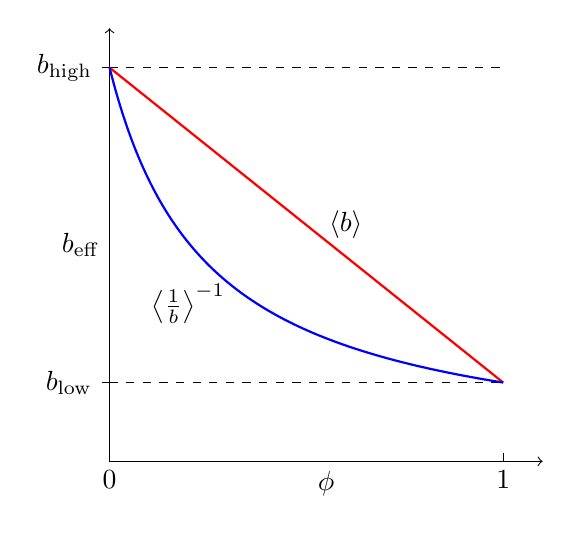
\begin{tikzpicture}

\draw[<->] (0,5.5) -- node[left]{\beff} (0,0) -- node[below]{$\phi$} (5.5,0);
\node at (0,0) [below]{0};
\node at (5,0) [below]{1};
\draw (5,0) -- ++(0,0.1);
\draw (0,1) -- ++(-0.1,0) node [left] {\blo};
\draw (0,5) -- ++(-0.1,0) node [left] {\bhi};

\draw[dashed] (0,1) -- ++(5,0);
\draw[dashed] (0,5) -- ++(5,0);

\draw[thick,red] (0,5) -- (5,1);
\draw[thick,blue] [domain=0:5,samples=200] plot (\x, {1/( (\x/5) *1  + (1-(\x/5))*0.2  )} );

\node at (3,3) {$\left< b \right>$};
\node at (1,2) {$\left< \frac{1}{b} \right>^{-1}$};

\end{tikzpicture}
\end{center}

The graph is possibly bad news for a nanoengineer: For surface tension to support water on top of air gaps, the air gaps must be quite narrow, hence period $L$ is very small.  Then it is likely that $L < \bmin$, so the harmonic mean formula applies, and therefore, $\beff$ is \textbf{dominated by the lowest slip present.}  The lower (blue) line of the graph shows that a large $\beff$ is achieved only with a very small fraction of low-slip surface.

Conversely, for macroscale patterning, one has $\bmax \ll L$, and so the simple mean formula applies.  In that case, any increase in the area of the high-slip region generates a proportional increase in $\beff$.


%\clearpage

\subsection*{Future Work}

We have mathematically rigorous results for $\beff$ in the opposing regimes $L \ll \bmin$ and $\bmax \ll L$.  Obviously, a complete theory of effective slip would present a rigorous formula that \textbf{interpolates} between the two extremes.  The graph above shows that the two formulae we present are upper and lower bounds on any hypothetical interpolating formula:  The formula (as a function of $\phi$) would have a curve lying somewhere between the two curves shown, depending on the ratio $b/ L$.  Finding such a formula is an obvious challenge for future work.

\vspace*{1em}

While the harmonic mean expression $\left< \frac{1}{b} \right>^{-1}$ is expected on mathematical grounds to be accurate when $L \ll \bmin$, numerical simulation reveals it to be rather good -- within 5\% -- even when $L$ and $b$ are similar.  At present, we cannot say why.  Another avenue for future work would be to attempt to rigorously quantify the error of $\beff$, as a function of $b/L$.

One clue is revealed in the 3-D flow surface plots: the velocity at the slip boundary does \emph{not} vary much, despite being subjected to varying boundary conditions.  It seems that the fluid does not have enough time to significantly speed up (or down) as the local slip length changes.  Perhaps quantifying the slip velocity variation as a function of $L$, $u$ and slip variation, would yield some insight.

\end{document}
